\documentclass[main.tex]{subfiles}

\begin{document}

\subsection{Primo esercizio}

 \includegraphics[width=\textwidth]{2015-0109-1.jpg}

\begin{alignat*}{5}
	R = 0.2\,m \quad
	AB = 0.55\,m \quad
	OG = 0.1\,m \quad
	M = 1\,Kg\quad
	J_G = 0.03\,Kgm^2
\end{alignat*}
\begin{alignat*}{5}
	m = 30\,kg\quad
	F = 1000\,N\quad
	v = 5\,m/s\quad
	a= 3\,m/s^2\quad
	\alpha = 45\,\deg
\end{alignat*}

Il sistema articolato rappresentato in figura è posto nel piano verticale. Il disco di caratteristiche note è incernierato a terra in O e ha baricentro in G. Il corsoio, di massa m e dimensioni trascurabili, si muove su una guida orizzontale liscia. Un’asta di massa trascurabile collega il punto A sulla circonferenza del disco al corsoio. Una forza $F$ nota è applicata sul corsoio. Assegnate la velocità $v$ e l’accelerazione a del corsoio (con i versi indicati in figura) si chiede di calcolare:

\begin{enumerate}
	\item La velocità e l’accelerazione angolare del disco (modulo e verso).
	\item La coppia $M_m$ da applicare al disco per garantire il moto assegnato.
\end{enumerate}

\clearpage

\subsection{Soluzione primo esercizio}

\subsubsection{Osservazioni importanti}

\begin{enumerate}
	\item Il baricentro del disco non coincide col centro geometrico. Questo generalmente comporta che la velocità del baricentro risulterà differente da quella del centro geometrico se il corpo ruota, come in questo caso. Questo porterà ad avere una componente di energia cinetica legata al moto traslatorio del baricentro, e non solo della rotazione momento d'inerzia baricentrico.
	\item Velocità ed accelerazione del punto B hanno verso discorde.
	\item Il CIR del disco è il punto O, che è vincolato a terra.
	\item La direzione della velocità del punto B, che è verso le ascisse positive, suggerisce una rotazione oraria del disco. Questo implica un valore negativo per la velocità angolare.
	\item La direzione dell'accelerazione del punto B, che è verso le ascisse negative, suggerisce un'accelerazione anti-oraria del disco. Questo implica un valore positivo per l'accelerazione angolare.
	\item La dimensione del segmento OB è variabile.
\end{enumerate}

\subsubsection{Primo punto}
Inizio scegliendo un'equazione di chiusura: (O-  A) + (A - B) = (O - B)

Risolvo con il metodo dei numeri complessi.

Inizio definendo, per quanto riguarda i segmenti, $a = OA$, $b = AB$ e $c = OB$ e per quanto riguarda gli angoli chiamo $\alpha$ l'angolo che determina la direzione di a e $\beta$ l'angolo che determina la direzione di b.

Inizialmente, $\alpha = \pi - \dfrac{\pi}{4} = \dfrac{3\pi}{4}$.

\begin{figure}[H]
\centering
\resizebox{.75\textwidth}{!}{% First image 2015 06 29

\begin{tikzpicture}

  \tiny

	\point{o}{0}{0};
  \point{a}{-1.4}{1.4};
  \point{b}{4}{0};
  \point{c}{4}{1.4};

	 \beam{2}{o}{a}[0][1];
	 \beam{2}{a}{b}[0][1];
	 \beam{2}{b}{o}[0][1];

	 \addon{3}{o}{a}{b}[-1];
	 %\addon{3}{c}{a}{e}[-1];
	 \addon{3}{a}{c}{b}[1];

	 \support{3}{o};

   %Degrees
   \notation{1}{o}{$\alpha$}[above];
   \notation{1}{a}{$\beta$}[above];

   \notation{5}{o}{a}[$a$];
   \notation{5}{a}{b}[$b$];
   \notation{5}{o}{b}[$c$];

\end{tikzpicture}}
\caption{Grafico semplificato}
\end{figure}

\paragraph{Spostamento}

\[
	ae^{i\alpha} + be^{i\beta} = c
\]

Scompongo in componenti cartesiane e calcolo il valore di $c$ e di $\beta$.

\[
	\begin{cases}
		a\cos\alpha + b\cos\beta = c\\
		a\sin\alpha + b\sin\beta = 0
	\end{cases}
	\Longrightarrow
	\begin{cases}
		c = a\cos\alpha + b\cos\beta\\
		\beta = \arcsin\left (-\dfrac{a\sin\alpha}{b}\right )
	\end{cases}
	\Longrightarrow
	\begin{cases}
		c = 0.39m\\
		\beta = -0.26\,rad
	\end{cases}
\]

I risultati ottenuti sono plausibili, sia dimensionalmente che nell'insieme dell'esercizio.

\paragraph{Velocità}

Derivo ed ottengo la velocità, ricordando che i termini che variano nel tempo sono $\alpha$, $\beta$ e $c$.

\[
	a\dot{\alpha}e^{i\left (\dfrac{\pi}{2} + \alpha \right )} + b\dot{\beta}e^{i\left (\dfrac{\pi}{2} + \beta \right )} = \dot{c}
\]

Scompongo in componenti cartesiane ed ottengo il valore di $\dot{\alpha}$ e $\dot{\beta}$:

\[
	\begin{cases}
		a\dot{\alpha}\sin\left (\dfrac{\pi}{2} + \alpha \right ) + b\dot{\beta}\sin\left (\dfrac{\pi}{2} + \beta \right ) = 0\\
		a\dot{\alpha}\cos\left (\dfrac{\pi}{2} + \alpha \right ) + b\dot{\beta}\cos\left (\dfrac{\pi}{2} + \beta \right ) = \dot{c}
	\end{cases}
	\Longrightarrow
	\begin{cases}
		a\dot{\alpha}\cos\left (\alpha \right ) + b\dot{\beta}\cos\left (\beta \right ) = 0\\
		-a\dot{\alpha}\sin\left (\alpha \right ) - b\dot{\beta}\sin\left (\beta \right ) = \dot{c}
	\end{cases}
\]

\[
\begin{cases}
	\dot{\alpha} = -\dfrac{b\dot{\beta}\cos\left (\beta \right )}{a\cos\left (\alpha \right ) } \\
	a\dfrac{b\dot{\beta}\cos\left (\beta \right )}{a\cos\left (\alpha \right ) }\sin\left (\alpha \right ) - b\dot{\beta}\sin\left (\beta \right ) = \dot{c}
\end{cases}
\Longrightarrow
\begin{cases}
	\dot{\alpha} = -\dfrac{b\dot{\beta}\cos\left (\beta \right )}{a\cos\left (\alpha \right ) } \\
	\dfrac{b\dot{\beta}\cos\left (\beta \right )}{\cos\left (\alpha \right ) }\sin\left (\alpha \right ) - b\dot{\beta}\sin\left (\beta \right ) = \dot{c}
\end{cases}
\]

\[
\begin{cases}
	\dot{\alpha} = -\dfrac{b\dot{\beta}\cos\left (\beta \right )}{a\cos\left (\alpha \right ) } \\
	\dot{\beta}b\left (\cos\left (\beta \right )\tan\left (\alpha \right ) - \sin\left (\beta \right )\right ) = \dot{c}
\end{cases}
\Longrightarrow
\begin{cases}
	\dot{\alpha} = -\dfrac{b\dot{\beta}\cos\left (\beta \right )}{a\cos\left (\alpha \right ) } \\
	\dot{\beta} = \dfrac{\dot{c}}{b\left (\cos\left (\beta \right )\tan\left (\alpha \right ) - \sin\left (\beta \right )\right )}
\end{cases}
\]

\[
\begin{cases}
	\dot{\alpha} = -48.2\,rad/s^2 \\
	\dot{\beta} = -12.8\,rad/s^2
\end{cases}
\]

I risultati ottenuti risultano plausibili, sia dimensionalmente che relativamente al moto del sistema in analisi.

\paragraph{Accelerazione}
Derivo nuovamente ed ottengo l'accelerazione, ricordando che i termini che variano nel tempo sono ora $\alpha$, $\beta$, $\dot{c}$, $\dot{\alpha}$, $\dot{\beta}$.

\[
	a\ddot{\alpha}e^{i\left (\dfrac{\pi}{2} + \alpha \right )} - a\dot{\alpha}^2e^{i\alpha} + b\ddot{\beta}e^{i\left (\dfrac{\pi}{2} + \beta \right )} -  b\dot{\beta}^2e^{i\beta} = \ddot{c}
\]

Scompongo in componenti cartesiane e risolvo per ottenere $\ddot{\alpha}$ e $\ddot{\beta}$:

\[
	\begin{cases}
		a\ddot{\alpha}\cos{\left (\dfrac{\pi}{2} + \alpha \right )} - a\dot{\alpha}^2\cos{\alpha} + b\ddot{\beta}\cos{\left (\dfrac{\pi}{2} + \beta \right )} -  b\dot{\beta}^2\cos{\beta} = \ddot{c} \\
		a\ddot{\alpha}\sin{\left (\dfrac{\pi}{2} + \alpha \right )} - a\dot{\alpha}^2\sin{\alpha} + b\ddot{\beta}\sin{\left (\dfrac{\pi}{2} + \beta \right )} -  b\dot{\beta}^2\sin{\beta} = 0
	\end{cases}
\]

\[
	\begin{cases}
		-a\ddot{\alpha}\sin{\alpha} - a\dot{\alpha}^2\cos{\alpha} - b\ddot{\beta}\sin{\beta} -  b\dot{\beta}^2\cos{\beta} = \ddot{c} \\
		a\ddot{\alpha}\cos{\alpha} - a\dot{\alpha}^2\sin{\alpha} + b\ddot{\beta}\cos{\beta} -  b\dot{\beta}^2\sin{\beta} = 0
	\end{cases}
\]

\[
	\begin{cases}
		-a\dfrac{a\dot{\alpha}^2\sin{\alpha} - b\ddot{\beta}\cos{\beta} +  b\dot{\beta}^2\sin{\beta}}{a\cos{\alpha}}\sin{\alpha} - a\dot{\alpha}^2\cos{\alpha} - b\ddot{\beta}\sin{\beta} -  b\dot{\beta}^2\cos{\beta} = \ddot{c} \\
		\ddot{\alpha} =  \dfrac{a\dot{\alpha}^2\sin{\alpha} - b\ddot{\beta}\cos{\beta} +  b\dot{\beta}^2\sin{\beta}}{a\cos{\alpha}}
	\end{cases}
\]

\[
	\begin{cases}
		(-a\dot{\alpha}^2\sin{\alpha} + b\ddot{\beta}\cos{\beta} -  b\dot{\beta}^2\sin{\beta})\tan{\alpha} - a\dot{\alpha}^2\cos{\alpha} - b\ddot{\beta}\sin{\beta} -  b\dot{\beta}^2\cos{\beta} = \ddot{c} \\
		\ddot{\alpha} =  \dfrac{a\dot{\alpha}^2\sin{\alpha} - b\ddot{\beta}\cos{\beta} +  b\dot{\beta}^2\sin{\beta}}{a\cos{\alpha}}
	\end{cases}
\]

\[
	\begin{cases}
		b\ddot{\beta}(\cos{\beta}\tan{\alpha} - \sin{\beta}) = \ddot{c} + b\dot{\beta}^2\cos{\beta} + a\dot{\alpha}^2\cos{\alpha} + b\dot{\beta}^2\sin{\beta}\tan{\alpha} + a\dot{\alpha}^2\sin{\alpha}\tan\alpha\\
		\ddot{\alpha} =  \dfrac{a\dot{\alpha}^2\sin{\alpha} - b\ddot{\beta}\cos{\beta} +  b\dot{\beta}^2\sin{\beta}}{a\cos{\alpha}}
	\end{cases}
\]

\[
	\begin{cases}
		\ddot{\beta} = \dfrac{\ddot{c} + b\dot{\beta}^2\cos{\beta} + a\dot{\alpha}^2\cos{\alpha} + b\dot{\beta}^2\sin{\beta}\tan{\alpha} + a\dot{\alpha}^2\sin{\alpha}\tan\alpha}{b(\cos{\beta}\tan{\alpha} - \sin{\beta})}\\
		\ddot{\alpha} =  \dfrac{a\dot{\alpha}^2\sin{\alpha} - b\ddot{\beta}\cos{\beta} +  b\dot{\beta}^2\sin{\beta}}{a\cos{\alpha}}
	\end{cases}
\]

Notando che $\ddot{c} = -a$ procedo con la sostituzione numerica:

\[
	\begin{cases}
		\ddot{\beta} = 1408.8\,rad/s^2\\
		\ddot{\alpha} =  3135.7\,rad/s^2 \quad (\ddot{\alpha}_{riportato} =  3131\,rad/s^2)
	\end{cases}
\]

\subsubsection{Secondo punto}

Per calcolare la coppa $M_m$ vado ad utilizzare il \textbf{bilancio delle potenze}.

\paragraph{Calcolo energia cinetica totale} Per calcolare l'energica cinetica totale identifico le masse in moto rotatorio o traslatorio, che in questo caso son sia il disco $M$ che il corsoio $m$.

\begin{center}
\framebox[4in]{
\begin{minipage}[t]{3.5in}
{\Large{\danger}} \textbf{N.B.}
Il baricentro \textit{non} coincide con il centro di rotazione del disco, per cui ha moto sia \textit{rotatorio} che \textit{traslatorio}. Per questo motivo, fornisce due componenti al bilancio dell'energia cinetica.
\end{minipage}}
\end{center}

\[
	E_c = \dfrac{1}{2}mv^2 + \dfrac{1}{2}Mv_G^2 + \dfrac{1}{2}J_G\dot{\alpha}^2
\]

Derivo questa espressione ed ottengo:

\[
	\dfrac{dE_c}{dt} = mv(-a) + Mv_Ga_G + J_G\dot{\alpha}\ddot{\alpha}
\]

Sostituisco tramite i legami cinematici $v_G$ e $a_G$:

\[
	\dfrac{dE_c}{dt} = M(-\dot{\alpha})(-\ddot{\alpha})OG^2 + J_G\dot{\alpha}\ddot{\alpha} -mva
\]

\[
	\dfrac{dE_c}{dt} = M\dot{\alpha}\ddot{\alpha}OG^2 + J_G\dot{\alpha}\ddot{\alpha} -mva
\]

\paragraph{Calcolo la potenza totale} Per calcolare la potenza totale, identifico le forze peso, le coppie, le forze degli attriti (statico, dinamico, volvente) e le forze applicate al sistema.

\begin{enumerate}
\item La forza peso applicata su B è controbilanciata da una forza normale del piano su cui giace il corsoio.
\item La forza peso agente su G, il baricentro del disco, non è controbilanciata. Il punto G si muove con una velocità $v_G = -\dot{\omega}OG$, che forma un angolo di $\dfrac{\pi}{2} + \dfrac{\pi}{4}$ con la forza peso.
\item La forza F agente su B ha direzione pari e verso opposto rispetto alla velocità $v$, forma quindi un angolo di $\pi$ con questo vettore.
\item La coppia $M_m$ ha verso opposto rispetto a $\dot{\alpha}$, per cui forma con questo vettore un angolo di $\pi$.
\end{enumerate}

\[
	\sum W_i = \vec{M_m}\bullet\dot{\alpha} +  \vec{F}_g\bullet\vec{v}_G + \vec{F}\bullet\vec{v}
\]

Risolvo il \textbf{prodotto scalare}:

\[
	\sum W_i = M_m\dot{\alpha}\cos\pi + F_gv_G\cos\left( \dfrac{\pi}{2} + \dfrac{\pi}{4} \right) + Fv\cos\pi
\]

\[
	\sum W_i = -M_m\dot{\alpha} - F_gv_G\sin\left( \dfrac{\pi}{4} \right) - Fv
\]

\paragraph{Uso il bilancio delle potenze}

\begin{equation}
	-M_m\dot{\alpha} - F_gv_G\sin\left( \dfrac{\pi}{4} \right) - Fv = M\dot{\alpha}\ddot{\alpha}OG^2 + J_G\dot{\alpha}\ddot{\alpha} -mva
\end{equation}

\begin{equation}
	-M_m\dot{\alpha}  = M\dot{\alpha}\ddot{\alpha}OG^2 + J_G\dot{\alpha}\ddot{\alpha} -mva + F_gv_G\sin\left( \dfrac{\pi}{4} \right) + Fv
\end{equation}

\begin{equation}
	M_m  = -\dfrac{M\dot{\alpha}\ddot{\alpha}OG^2 + J_G\dot{\alpha}\ddot{\alpha} -mva + F_gv_G\sin\left( \dfrac{\pi}{4} \right) + Fv}{\dot{\alpha}}
\end{equation}

\begin{equation}
	M_m  = -\dfrac{M\dot{\alpha}\ddot{\alpha}OG^2 + J_G\dot{\alpha}\ddot{\alpha} -mva + Mg(-OG\dot{\alpha})\sin\left( \dfrac{\pi}{4} \right) + Fv}{\dot{\alpha}}
\end{equation}

\begin{equation}
	M_m = -30.26\,Nm \quad (M_{m_{riportato}} = -30.1\,Nm)
\end{equation}


\end{document}